% -*- TeX:SI -*-
% slovene sub-mode for spell check
%%%%%%%%%%%%%%%%%%%%%%%%%%%%%%%%%%%%%%%%%%%%%%%%%%%%%%%%%%%%%%%%%%%%%%%%%%%%%%%%%%%%%%%%%%%%%%%%%%%%%%%%%%%%%%%%%%%%%%%%
% LaTeX predloga za zaključna dela
% Univerza v Ljubljani, Fakulteta za elektrotehniko
% Zbral in uredil: Roman Kamnik, junij 2013
% Dopolnil: Sebastjan Šlajpah (2013), Sašo Tomažič (2013), Peter Miklavčič (2019)
%%%%%%%%%%%%%%%%%%%%%%%%%%%%%%%%%%%%%%%%%%%%%%%%%%%%%%%%%%%%%%%%%%%%%%%%%%%%%%%%%%%%%%%%%%%%%%%%%%%%%%%%%%%%%%%%%%%%%%%%
\documentclass[a4paper,twoside,openright,12pt,slovene]{book}
\usepackage[pdftex]{UNI-LJ-FE-Diploma} % stil zaključnega dela UL FE
\usepackage[utf8]{inputenc} % predloga uporablja standardno kodiranje Unicode UTF-8, ki podpira šumnike
\usepackage[greek,english,slovene]{babel} % seznam uporabljenih jezikov (zadnji na seznamu je primarni)

% PDF/A %%%%%%%%%%%%%%%%%%%%%%%%%%%%%%%%%%%%%%%%%%%%%%%%%%%%%%%%%%%%%%%%%%%%%%%%%%%%%%%%%%%%%%%%%%%%%%%%%%%%%%%%%%%%%%%%
% Več o PDF/A v LaTeX-u: https://www.mathstat.dal.ca/~selinger/pdfa/
\usepackage{filecontents}
\begin{filecontents*}{\jobname.xmpdata}
    \Title{Asinhrona sekvenčna digitalna vezja} % Mora biti enak kot je v prijavi teme!
    \Author{Gal Nadrag} % Mora biti enak kot na naslovnici!
\end{filecontents*}
\usepackage[a-1b]{pdfx}
%%%%%%%%%%%%%%%%%%%%%%%%%%%%%%%%%%%%%%%%%%%%%%%%%%%%%%%%%%%%%%%%%%%%%%%%%%%%%%%%%%%%%%%%%%%%%%%%%%%%%%%%%%%%%%%%%%%%%%%%

% LaTeX PAKETI %%%%%%%%%%%%%%%%%%%%%%%%%%%%%%%%%%%%%%%%%%%%%%%%%%%%%%%%%%%%%%%%%%%%%%%%%%%%%%%%%%%%%%%%%%%%%%%%%%%%%%%%%
% Kompakten pregled LaTeX ukazov je dostopen na https://en.wikibooks.org/wiki/Category:Book:LaTeX
% Navodila posameznih uporabljenih paketov so dostopna na https://www.ctan.org

% Dodatni simboli
\usepackage{textcomp}                               % dodatni simboli (kot npr. €)
\usepackage{gensymb}                                % dodatni simboli \de­gree, \cel­sius, \pert­hou­sand, \mi­cro, \ohm
\newcommand{\uppi}{\textrm{\greektext p\latintext}} % velika grška črka P z \uppi, alternativa simbolu \Pi

% Osnovno oblikovanje
\hypersetup{unicode,hidelinks,breaklinks,hyperindex} % dodatne možnosti hiperpovezav
\usepackage[normalem]{ulem}                          % podčrtavanje in prečrtavanje teksta
\usepackage{float}                                   % dodatne možnosti oblikovanja objektov
\usepackage{enumitem}                                % dodatne možnosti oblikovanja seznamov

% Dodatno oblikovanje
%\zamaknirobsodihstrani{0mm} % dodatna prilagoditev levega roba sodih strani za dvostranski tisk
%\usepackage{dcolumn}        % poravnava po decimalnih mestih v tabelah
%\usepackage{longtable}      % večstranske tabele
%\usepackage{caption}        % dodatne možnosti označevanja objektov
%\usepackage{rotating}       % vretenje objektov, strani, ipd.

% Matematična orodja
\usepackage{mathtools} % http://mirrors.ctan.org/macros/LaTeX/contrib/mathtools/mathtools.pdf
\usepackage{bm}        % ukaz za odebeljeni tisk \bm v matematičnih okoljih
%\usepackage{cancel}   % ukaz za prečrtavanje \cancel v matematičnih okoljih

% Grafična orodja
\usepackage{graphicx}                 % vključevanje bitnih slik z ukazom \includegraphics
\usepackage{grffile}                  % podpora presledkom pri ukazu \includegraphics
%\usepackage{tikz}                    % paket TikZ za risanje (npr. blokovnih shem, diagramov poteka, itd.)
%\usetikzlibrary{calc,shapes,arrows}  % dodatne možnosti paketa TikZ
%\usepackage{tikzscale}               % skaliranje risb
%\usepackage[smartlabels]{circuitikz} % risanje shem vezij
%\usepackage{pgfplots}                % paket PGFPlots za risanje grafov, tudi iz CSV in podobnih datotek
%\usepgfplotslibrary{polar,external}  % dodatne možnosti paketa PGFPlots
%\usepackage{tikz-3dplot}             % 3D risanje
% Primeri: http://texample.net , http://pgfplots.net/tikz/examples , http://pgfplots.sourceforge.net/gallery.html

% Vključevanje datotek
\usepackage{pdfpages} % vključevanje PDF datotek z ukazom \includegraphics
\usepackage{epstopdf} % vključevanje EPS datotek z ukazom \includegraphics
\usepackage{listings} % orodja za izpisovanje programske kode
\lstset{              % nastavitve orodja za izpisovanje programske kode
    basicstyle=\ttfamily\footnotesize,
    breaklines=true,
    numbers=left,
    numberstyle=\scriptsize,
    keywordstyle=\color{blue},
    commentstyle=\color{unilj},
    stringstyle=\color{olive},
}
%%%%%%%%%%%%%%%%%%%%%%%%%%%%%%%%%%%%%%%%%%%%%%%%%%%%%%%%%%%%%%%%%%%%%%%%%%%%%%%%%%%%%%%%%%%%%%%%%%%%%%%%%%%%%%%%%%%%%%%%

% DEKLARACIJE %%%%%%%%%%%%%%%%%%%%%%%%%%%%%%%%%%%%%%%%%%%%%%%%%%%%%%%%%%%%%%%%%%%%%%%%%%%%%%%%%%%%%%%%%%%%%%%%%%%%%%%%%%
\naslov{Asinhrona sekvenčna digitalna vezja} % Mora biti enak kot je v prijavi teme!
\avtor{Gal Nadrag} % Mora se ujemati s \Title pri metapodatkih PDF/A!
\mentor{Aleksander Sešek}
%\somentor{Naziv, ime in priimek somentorja}
\date{Ljubljana, \the\year}
\univerza{Univerza v Ljubljani}
\definecolor{unilj}{cmyk}{0.00, 0.94, 0.94, 0.06} % barva Univerze v Ljubljani

% Potrebno je paziti, da je izbrana prava kombinacija tipa dela in sodelujočih fakultet glede na študijski program!
%\delo{Diplomsko delo\\~\\Univerzitetni študijski program prve stopnje Elektrotehnika}
%\delo{Diplomsko delo\\~\\Univerzitetni študijski program prve stopnje Multimedija}
%\delo{Diplomsko delo\\~\\Visokošolski strokovni študijski program\\prve stopnje Aplikativna elektrotehnika}
%\delo{Diplomsko delo\\~\\Visokošolski strokovni študijski program\\prve stopnje Multimedijske komunikacije}
\delo{Magistrsko delo\\~\\Magistrski študijski program druge stopnje Elektrotehnika}
%\delo{Magistrsko delo\\~\\Magistrski študijski program druge stopnje Uporabna statistika}
\fakulteta{Fakulteta za elektrotehniko}
%\fakulteta{Fakulteta za elektrotehniko,\\Fakulteta za računalništvo in informatiko} % Za program Multimedija
%\fakulteta{Fakulteta za elektrotehniko, Biotehniška fakulteta,\\Ekonomska fakulteta, Fakulteta za družbene vede,\\Fakulteta za matematiko in fiziko, Fakulteta za\\računalništvo in informatiko, Medicinska fakulteta} % Za program Uporabna statistika
%%%%%%%%%%%%%%%%%%%%%%%%%%%%%%%%%%%%%%%%%%%%%%%%%%%%%%%%%%%%%%%%%%%%%%%%%%%%%%%%%%%%%%%%%%%%%%%%%%%%%%%%%%%%%%%%%%%%%%%%

% DOKUMENT %%%%%%%%%%%%%%%%%%%%%%%%%%%%%%%%%%%%%%%%%%%%%%%%%%%%%%%%%%%%%%%%%%%%%%%%%%%%%%%%%%%%%%%%%%%%%%%%%%%%%%%%%%%%%
\begin{document}
\frontmatter

\selectlanguage{slovene}

%******************************* NASLOVNICA ************************************
\maketitle

%******************************* ZAHVALA ***************************************
% -*- TeX:SI -*-
% Zahvala
\vspace*{0mm}
\Large\textbf{Zahvala}\normalsize
\vskip\medskipamount % or other desired dimension
\leaders\vrule width \textwidth\vskip0.4pt % or other desired thickness
\vskip\bigskipamount % ditto


[Pisanje zahvale ali posvetila je neobvezno.]

[Pri zahvali napišite zahvalo tistim, ki so pomagali pri nastanku dela in brez katerih delo ne bi nastalo v takšni obliki, kot je. Navadno se je potrebno zahvaliti v prvi vrsti mentorju, somentorju in inštituciji, ki je morda finančno ali kako drugače podprla izvedbo zaključnega dela. Nato sledijo asistenti, ostali sodelavci in vaši kolegi, ki so pomagali pri teoretičnem in eksperimentalnem delu. Na koncu se po navadi zahvalimo še družini.]


\newpage
%******************************* POVZETEK IN KLJUČNE BESEDE ********************
%******************************* POVZETEK IN KLJU?NE BESEDE ********************
\povzetek
V zadnjem desetletju smo bili priča prenehanju povečevanja taktnih frekvenc posameznih procesorskih jeder. A hkrati število tranzistorjev še vedno narašča. Trenutni trend je povečevanje števila jeder, vendar nekaterih problemov ni mogoče paralelizirati, zato ta pristop ne pomaga.

V tem delu predstavljamo metodo za načrtovanje asinhronih digitalnih vezij. Ta vezja ne potrebujejo taktnega signala in so hitrostno omejena le z omejitvami vrat in povezav. Predstavljamo tudi metodo za implementacijo takšnih vezij v FPGA. Implementacije osnovnih vezji doežejo efektivne frekvenco 35MHz.

\kljucnebesede
Asinhrona logika, Digitalna logika, FPGA

\newpage
%******************************* ABSTRACT AND KEYWORDS *************************
%******************************* ABSTRACT AND KEYWORDS *************************
\selectlanguage{english}

\abstract
In the last decade, we have witnessed the cessation of the increase in clock frequency of individual processor cores. At the same time, the number of transistors continues to grow. The current trend is to increase the number of cores, but some problems cannot be parallelized, so this approach does not help.

In this work, we present a method for designing asynchronous digital circuits. These circuits do not require a clock signal and are speed-limited only by gate and connection constraints. We also present a method for implementing such circuits in FPGA. Implementations of basic cirucits reach effective frequencies of 35MHz.

\keywords
Asynchronous logic, Digital logic, FPGA

\selectlanguage{slovene}

\newpage
%******************************* KAZALO ****************************************
\tableofcontents

%******************************* SEZNAM SLIK, SEZNAM TABEL *********************
\seznamslik
\seznamtabel

%******************************* SEZNAM SIMBOLOV *******************************
%******************************* SEZNAM SIMBOLOV IN KRATIC *******************************
\seznamsimbolovinkratic
V pričujočem zaključnem delu so uporabljene naslednje veličine in simboli:

\begin{center}
	\begin{tabular}{*{2}{l}} 
		\hline
		\bf{Kratica}        & \bf{Pomen}    					\\ 
		\hline
		FPGA                & Field programmable gate array		\\
		STG                 & State transition graph			\\
		DFS                 & Dataflow structure			\\
		\hline
	\end{tabular}
\end{center}

\begin{center}
	\begin{tabular}{*{4}{l}} \hline
		\multicolumn{2}{c}{\bf{Veličina / oznaka}}          & \multicolumn{2}{c}{\bf{Enota}} 	\\ 
		\hline
		Ime                & Simbol                         & Ime      			& Simbol              	\\ 
		\hline
		čas                & $t$                            & sekunda  			& s                   	\\
		frekvenca          & $f$                            & Hertz    			& Hz                  	\\
		napetost           & $U$                         	& Volt        		& V		            	\\
		tok                & $I$                            & Amper 			& A                  	\\
		kapacitivnost      & $C$                   			& Farad     		& F                   	\\
		\hline
	\end{tabular}
\end{center}




\newpage
\mainmatter
%******************************* UVOD ******************************************
%******************************* UVOD ******************************************
\chapter{Uvod} \label{uvod}

Digitalna vezja uporabljamo za obdelavo podatkov. Osnovna digitalna vezja glede na vhodne podatke naredijo izhodne podatke, torej nimajo spomina. Taka vezja imenujemo \textbf{kombinatorična} vezja.
Z kombinatoričnimi vezji lahko izračunamo kar koli želimo a imamo težavo:

\textbf{Velikost}: velikost kombinatoričnega vezja je v splošnem proporcionalna kvadratu števila vhodov in proporcionalna številu izhodov. Ker želimo obdelovati gigabajte podatkov in več je to jasno nesprejemljivo.

Rešitev je, da kose vezja uporabimo večkrat, torej da naredimo povratno vezavo. Izhod takih vezji ni več odvisen le od vhodov, temveč tudi od stanja povratne zanke, torej imajo taka vezja spomin, imenujejo se \textbf{sekvenčna} vezja.

Ampak tu se pojavi nova težava. Predstavljajmo si seštevalnik, katerega izhod povežemo na enega izmed vhodov, Na drugi vhod damo konstanto 1.
Želeli bi si, da vezje šteje 1,2,3... Ampak to se ne zgodi, namesto tega na izhodu dobimo kaotične signale. Razlog je, da je v vezju ogromno število povratnih zank, vendar med seboj niso sinhronizirane. Zato zanke počasi zlezejo iz faze in na izhodu dobimo šum.

Nujno je torej vpeljati mehanizem s katerim periodično sinhroniziramo povratne zanke. To storimo s spominskimi elementi, ki jih vstavimo v povratno vezavo, rečemo jim \textbf{registri}. Registri ne smejo prepustiti naprej novih podatkov, dokler niso stari podatki popolnoma obdelani. Efektivno ponovno sinhronizirajo faze vseh povratnih zank.

Torej moramo izvedeti kdaj so podatki na vhodu registra obdelani, in podatki trenutno v registru obdelani. Takrat lahko register sprejme nove podatke.

V splošnem imamo dva načina na katera lahko storimo:

-Globalna sinhronizacija(Urin takt):
	V tej shemi uporabimo predpostavko, da obdelva podatkov v \textbf{vseh} vezjih med dvema zaporednima registroma ne traja dlje od neke konstante. Vse registre nato naenktrat sinhroniziramo z to periodo. To naredimo z urinim taktom. Footnote: Urin takt je generiran prek kristalnega oscilatorja ali RC oscilatorja. Vse povratne zanke v vezju nato sinhronizirano z tem oscilatorjem, ki mora imeti najdaljšo periodo.
	
-Lokalna sinhronizacija
	V tej shemi sinhroniziramo vse povratne zanke na en signal. Zagotoviti moramo, da ima ta signal \textbf{najdaljšo} periodo izmed vseh povratnih zank. 




	

\newpage
%******************************* POGLAVJA **************************************
%******************************* POGLAVJA **************************************
\chapter{Teoretične osnove} \label{osnove}

Da bomo lahko asinhrona vezja analizirali in zasnovali potrebujemo povzeti teoretične osnove s katerimi taka vezja modeliramo. Moramo se naučiti kako v takih vezjih signali potujejo in kako dosežemo, da potujejo urejeno. 


\section{Asinhroni koncepti} \label{a}
V sinhronih vezjih taktni signal določa časovne točke, kjer so signali v vezju veljavni. Ker v asinhronih vezjih nimamo taktnega signala, morajo biti vsi signali vedno veljavni. Zato proučujemo naša vezja na nivoju sprememb.
Sprememba je prehod nekega signala iz stanja 1 v stanje 0 ali obratno. Potovanje sprememb skozi naše vezje določa njegovo delovanje. Da asinhron sistem deluje pravilno mora slediti naslednjim pravilom.

\begin{itemize}
	\item Spremembe se ne pojavljajo iz nikoder.
	\item Spremembe ne izginjajo.
\end{itemize}

Da se spremembe ne smejo zgoditi brez razloga je jasno nujno, saj sicer vrednost podatkov ni nujno pravilna. Obstajajo vezja, ki delujejo v ekstremnih pogojih npr. v vesolju, kjer lahko šum inducira spremembe napetostnih nivojev v vezju. Taka vezja potrebujejo redundantne kopije, da zagotovijo pravilnost izračunov.

Konceptu, da spremembe ne smejo izginjati pravimo \textbf{indikacija}.

\subsection{Indikacija} \label{b}

Indikacija je pomemben koncept pri asinhronih vezjih. Signal je indiciran, če ima vsaka njegova sprememba posledice. Prestavljajmo si ALI logična vrata. Recimo, da je stanje na vhodu
\[[0,0] \mapsto 0\]
Če en signal preklopi, se spremeni stanje izhoda, torej ima sprememba posledice.
\[[0,\color{red}1\color{black}] \color{red}\mapsto 1\]
Če sedaj preklopi še drugi signal, se stanje na izhodu ne spremeni .
\[[\color{red}1\color{black},1] \mapsto 1\]
To pomeni, da ne vemo če se je drugi signal že spropagiral od vira. Po drugi strani, če originalni signal preklopi nazaj, se izhod ponovno spremeni.
\[[0,\color{red}0\color{black}] \color{red}\mapsto 0\]
Če ne želimo uporabljati časovnih predpostavk, mora vsaka sprememba vsakega signala biti indicirana. To pomeni, da mora na vhodu ALI in IN vrat signal vedno preklopiti dvakrat zaporedno, na vhodu C elementa morata signala preklopiti eden za drugim itd. 

\begin{figure}[H]
	\centering
	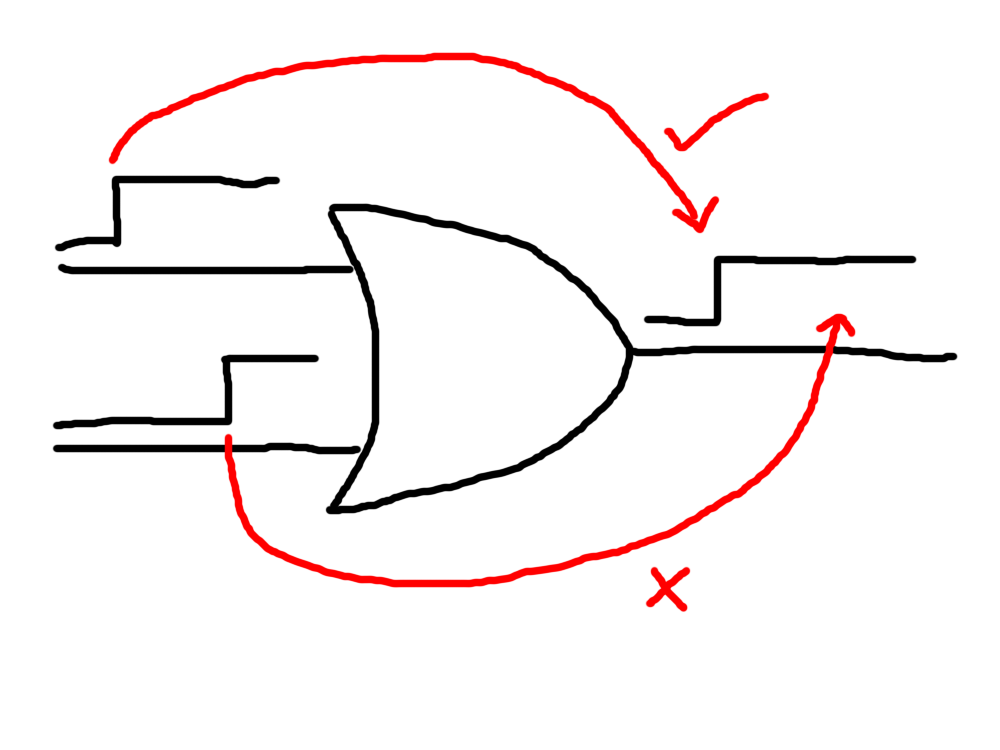
\includegraphics[width=0.7\linewidth]{slike/osnove/indication}
	\caption{}
	\label{fig:celement}
\end{figure}




\subsection{Hitrostna neodvisnost} \label{b}
Naredimo model asinhronih vezji, da bolje razumemo kako delujejo. Predstavljajmo si vezje vrat, povezanih med seboj. Vsaka vrata imajo vhodne in izhodne signale. Ko vhod vrat diktira spremembo izhoda postanejo vrata aktivna. Po neznanem časovnem zamiku se spremeni tudi izhod. Zanimivo je, kar se zgodi na izhodu vrat. Vrata ki imajo na vhodu izhodni signal naše originalnih vrat imajo tri opcije.
Lahko sprememba vhoda ne spremeni izhoda.
Lahko sprememba vhoda ne povzroči spremembe izhoda.
Lahko pa so bila vrata aktivna, a zaradi spremembe izhoda sedaj niso več aktivna.

Asinhrona vezja delujejo pravilno, če se zadnji kriterij nikoli ne zgodi.

Obstajajo različni razredi asinhronih vezji, kjer je ta kriterij realiziran z različnimi predpostavkami.

\subsection{Hitrostna neodvisnost} \label{b}
Hitrostno neodvisna vezja imajo neznane zakasnitve v vratih in nimajo zakasnitev v žicah. To žal ni zelo realno v današnjih vezjih, kjer so zakasnitve v žicah lahko velik del zakasnitve v logičnih vejah. Še posebej pa to ne velja v FPGA, zato ta vezja niso zelo zanesljiva.

\subsection{Zakasnilna neodvisnost} \label{b}

Vezja, ki so neodvisna na zakasnitve imajo neznane zakasnitve v žicah in vratih, tu ne predpostavimo nič, ampak S takimi vezji ne moremo procesirati podatkov. Citat

\subsection{Kvazi-zakasnilna neodvisnost} \label{b}
Srednja pot je kvazi zakasnitvena neodvisnost, kjer imamo določene predpostavke, o zakasnitvah v le določenih žicah.







\section{Sinhronizacija} \label{a}
Sinhronizacija je pojav, kjer dva procesa delita informacije, da delita neko vrednost. V našem primeru je ta vrednost perioda.

\subsection{Muller C element} \label{c}
Muller C element je osnovni element sinhronizacije dveh signalov. Ima dva vhoda, izhod se spremeni, ko sta oba vhoda enaka.

\begin{figure}[H]
	\centering
	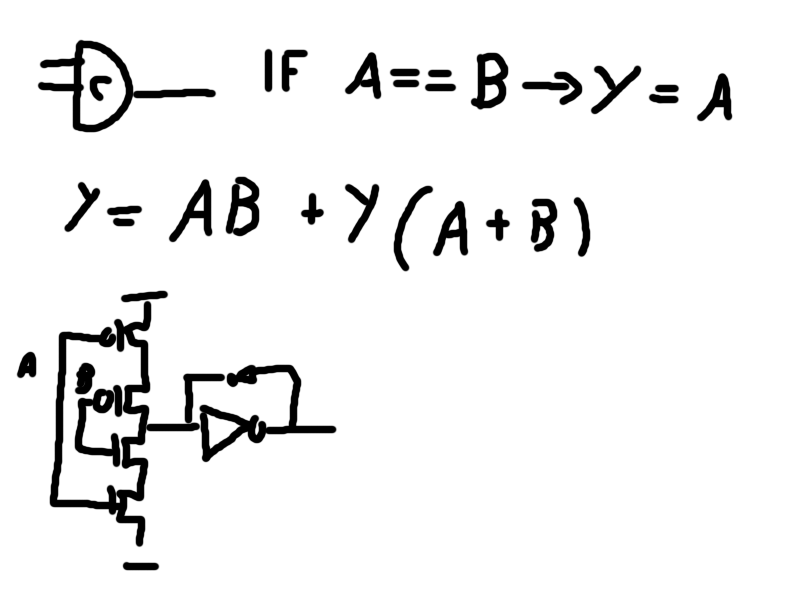
\includegraphics[width=0.7\linewidth]{slike/osnove/C_Element}
	\caption{}
	\label{fig:celement}
\end{figure}



\section{Združevanje} \label{a}
Ko združimo poti dveh signalov, na izhodu dobimo izhod, če je na vhodu katerikoli od vhodnih signalov. Je ALI funkcija za signale.

\section{Multiplekser} \label{a}
Izbira en signal šofira po dveh poteh. Izbiro poti lahko nadzira zunanji signal. To je multiplekser signalov

\section{Razcepljanje} \label{a}
Razcepljanje je preprosta duplikacija izhodnih signalov.


\section{Osnovna vezja} \label{b}
Najosnovnejše vezje, ki ima periodo je obročni oscilator. Obročni oscilator je narejen iz inverterja, ki povzroči negativno povratno zanko in zakasnilne linije, ki določa periodo oscilatorja.

Začnimo torej z sinhronizacijo dveh obročnih oscilatorjev. Za ta namen potrebujemo posebna logična vrata.

Poglejmo si kako tak element sinhronizira dva signala:

\subsection{Vzporedna sinhronizacija} \label{c}

Imamo dve povratni zanki, vsaka z različno zakasnitvjo, kateri želimo sinhronizirati.

\begin{figure}[H]
	\centering
	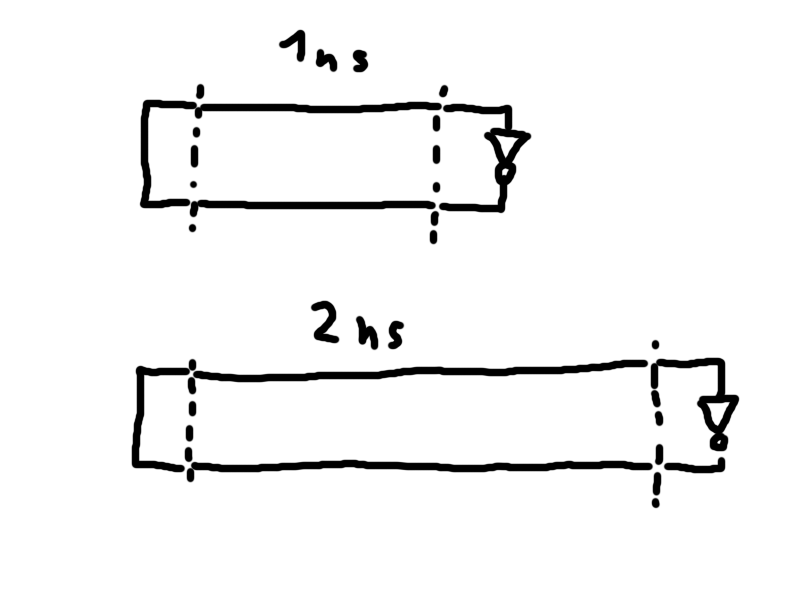
\includegraphics[width=0.7\linewidth]{slike/osnove/dly1}
	\caption{}
	\label{fig:celement}
\end{figure}

Če ustvarimo prek C elementa skupno povratno zanko, mora hirejši vedno čakati počasnejšega, torej sta sinhronizirana.

\begin{figure}[H]
	\centering
	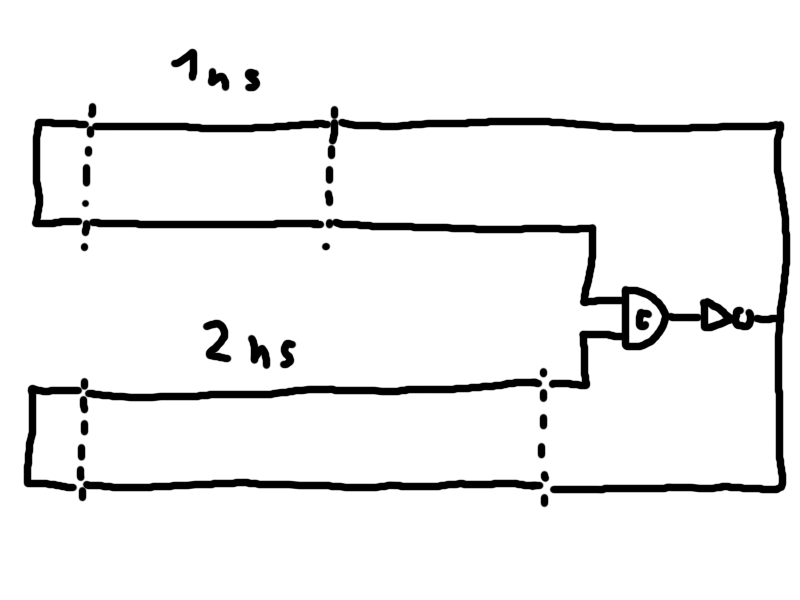
\includegraphics[width=0.7\linewidth]{slike/osnove/dly2}
	\caption{}
	\label{fig:celement}
\end{figure}

Trivialno lahko sinhroniziramo poljubno število povratnih zank.

\begin{figure}[H]
	\centering
	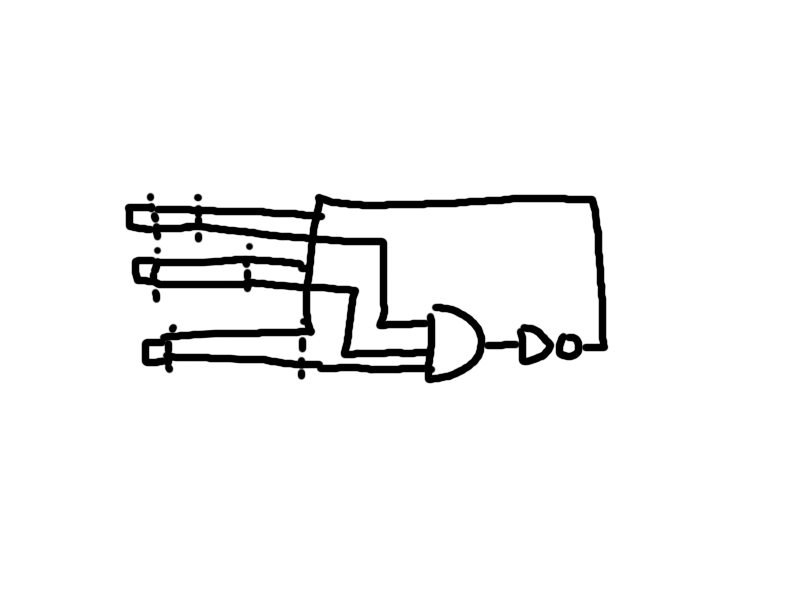
\includegraphics[width=0.7\linewidth]{slike/osnove/dly3}
	\caption{}
	\label{fig:celement}
\end{figure}

To lahko razumemo kot vzporedno vezavo oscilatorjev, kjer je skupna perioda, perioda najdaljše povratne zanke. 

\subsection{Zaporedna sinhronizacija} \label{c}
Lahko pa vežemo oscilatorje tudi zaporedno na sledeči način:

%Inverter na napacni strani

\begin{figure}[H]
	\centering
	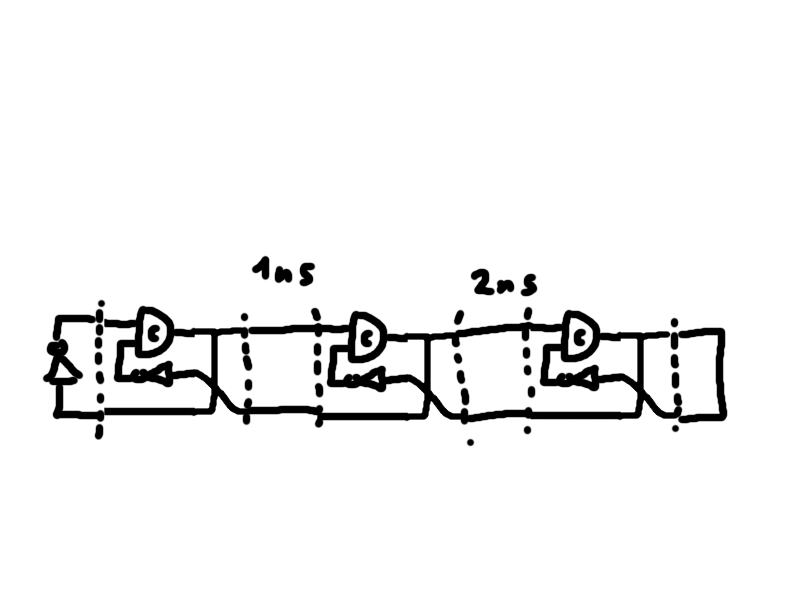
\includegraphics[width=0.7\linewidth]{slike/osnove/dly4}
	\caption{}
	\label{fig:celement}
\end{figure}

Tu povratne zanke prepletemo med seboj. Vsako povratno zanko sprožijo njeni sosedje. V tem primeru prva zanka sproži drugo. Ko druga konča ponovno sporži prvo.

Tak vzorec lahko nadaljujemo poljubno dolgo.
\begin{figure}[H]
	\centering
	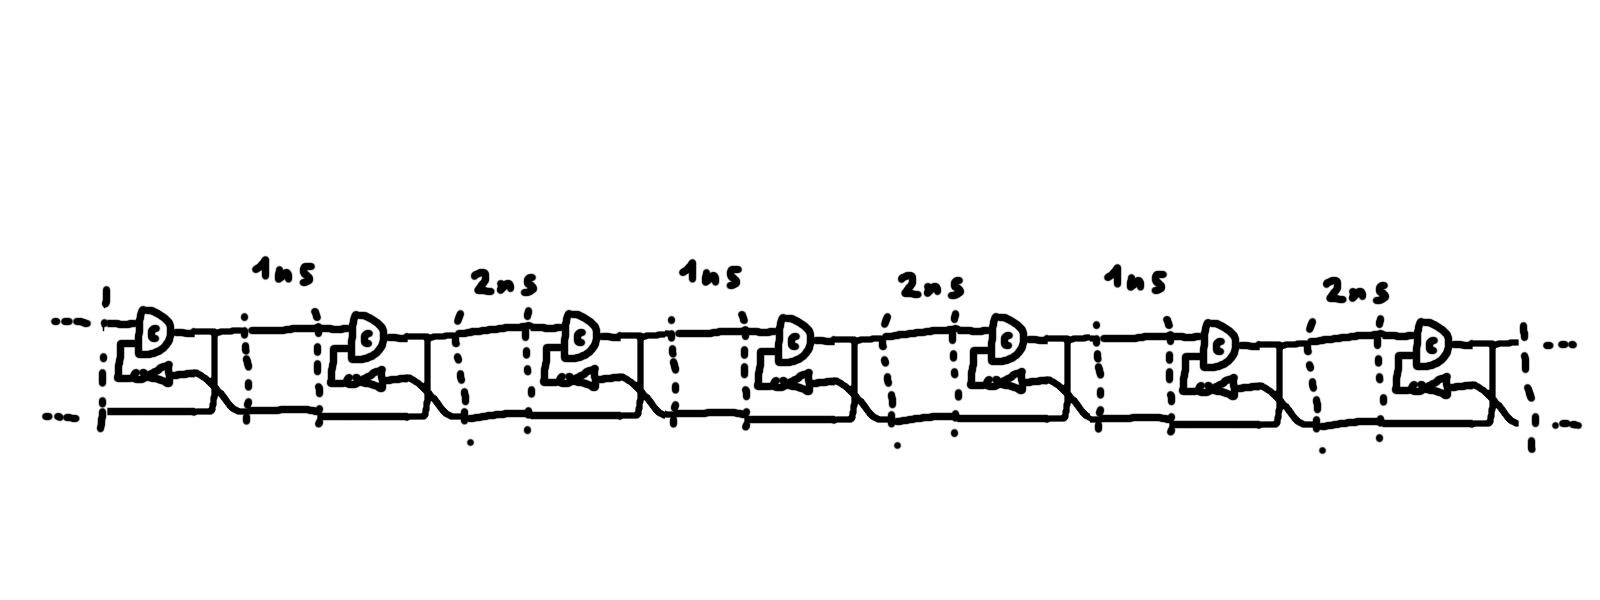
\includegraphics[width=0.7\linewidth]{slike/osnove/dly5}
	\caption{}
	\label{fig:celement}
\end{figure}






\chapter{Zasnova asinhronih vezji} \label{zasnova}

Če želimo zasnovati asinhrona vezja moramo zasnovati visoko nivojski pogled, podobno kot pri sinhronih vezjih. Pri sinhronih vezjih je osnovna dogma to, da imamo zaporedje registrov in logike med njimi. Na vsak pozitivni rob urinega takta, se podatki prenesejo za en register naprej. To nam dovoli, da poenostavimo zasnovo sinhronih digitalnih vezji na zaporedje matematičnih operacij.

Podobno lahko storimo tudi pri asinhronih vezjih, imamo dodatne omejitve. Še vedno imamo zaporedje registrov, ter logiko med njimi, vendar se sedaj podatki ne pretakajo periodično, zato moramo zagotoviti da ne pride do zastojev.

\section{Protokoli} \label{a}

Najprej poglejmo kako podatke prenašamo skozi asinhrona vezja. Na sploh se protokoli deljio v dve skupini po dve skupini.

\subsection{Faznost} \label{b}

\begin{itemize}
	\item 2phase hitrejsi, ampak rabimo feedback da vemo kdaj smo done
	\item 4phase preprostejši več komunikacije
\end{itemize}

Pomislimo na mullerjev cevovod. Prenos podatkov po njem lahko gledamo na dva načina.
Lahko gledamo na nivoje signalov. Cikel torej gre reqdata, ackdata, reqnull, acknull. V tem pogledu potujeta skozi cevovod dva valova. Prvi je podatkovni val, ki prenaša podatke. Drugi je zaključni val, ki zakjuči komunikacijo, in spravi kanal v prvotno stanje.

Lahko gledamo robove signalov. Torej gledamo prenos dogodkov (pozitivni in negativni rob imata enak pomen). Torej gre samo za podatkovne valove, ki sledijo eden drugemu.


\subsection{Podatki} \label{b}

\begin{itemize}
	\item bundled data: Podoben sinhronim vezjem, potrebuje zakasnitve, da zagotovimo časovne predpostavke.
	\item Dual rail: Dve žici na bit, manj predpostavk
\end{itemize}

Do sedaj smo gledali cevovod le kot 1 biten podatkovni kanal. Vendar za procesiranje podatkov želimo več-bitne podatke. Cevovod lahko posplošimo na dva načina. 

Lahko signale, ki potujejo po cevovodu uporabimo, za odpiranje klasičnih registrov. To pomeni da lahko uporabimo klasične registre in klasično logiko. Vendar moramo paziti, da ohranimo pot skozi cevovod najdaljšo, torej potrebujemo zakasnilne elemente.

Lahko sklopimo več cevovodov skupaj. Med seboj moramo povezati povratne zanke in poskrbeti, za pravo kodiranje podatkov.

\subsubsection{Kodiranje} \label{b}
Kot vemo, moramo poskrbeti, da povratno zanko sinhroniziramo na najpočasnejši signal v zanki. To lahko zagotovimo z pravilnim kodiranjem podatkov. Koda je neodvisna od zakasnitev ko nobena kodna beseda ni vključena v drugi kodni besedi. Želimo tudi da je konkatanacija dveh kodnih besed nova kodna beseda.

Imamo dva jasna kandidata

\begin{itemize}
	\item One hot quad.
	\item Dual rail: One hot dual
\end{itemize}

One hot quad ima enako podatkovno gostoto kot dual rail, vendar ima pol manj preklopov, kar jo naredi bolj energisjko učinkovito. Vendar nismo še našli učinkovitih impelmentacij. Zato uporabimo Dual rail.

%
%A code (I ,C) is called delay-insensitive when :MATH @ dicodes:that is, when no code word is contained in another code word
%

Glede na gornje izbire dobimo 4 načine implementacije asinhronih vezji. Poglejmo si osnove vseh ter pogledjmo prednosti in slabosti.

\subsection{4-Phase bundled data} \label{b}
Ta stil je najbolj podoben klasični sinhroni logiki. Uporablja Mulerjev cevovod kot osnovno vodilo podatkovnega poteka. Na ta cevovod pripnemo navadne zapahe skozi katere pretekajo podatki. Med zapahe lahko vstavimo klasično logiko, a moramo paziti, da vsatvimo v Mullerjev cevovod zadostne zakasnitve, da zagotovimo dovolj časa, da se signali propagirajo skozi logiko. Ker je protokol 

\subsection{2-Phase bundled data} \label{b}
Ta stil je podoben 4-Phase bundled data, saj enako uporablja Mullerjev cevovod kot vodilo podatkov in klasično logiko. Ker uporablja 2 fazni protokol predstavljajo preklopi na cevovodu podatke o stanju cevovoda. Zato potrebujemo posebne zapahe, ki so odprti, ko sta stanja trenutne in naslednje stopnje cevovoda različni, sicer pa je zaprt. Tak protokol je hitrejši in bolj energetsko učikovit, prednost je tudi, da ne potrebujemo asimetričnih zakasnitev. Slabost so tudi posebni zapahi, ki niso del večine knjižnjic.

\subsection{4-Phase dual rail} \label{b}
Ta stil uporablja dual rail komunikacijo, kar prinese veliko overhead saj moramo uporabiti dvakrat več linij za podatkovne povezave in moramo vgraditi spominske celice v samo kombinatorično logiko. Druga stran je izjemna zanesljivost protokola, ki je dosežena popolnoma brez zakasnitev. Edina časovna predpostavka so nekatere isohronične veje, ki so zelo lahko izpolnjene

\subsection{2-Phase dual rail} \label{b}
Ta magisterska naloga se nanaša na implementacijo tega stila komunikacije. Je podoben 4-Phase dual rail, ampak namesto uporablja 2 fazni protokol, torej pridobimo na hitrosti in energijski učinkovitosti. Slabost je, da je povšina takšne izvedbe daleč največja. V nadaljnih poglavjih, se fokusiramo na prednosti in slabosti tega stila, ter njegovi detajli.




\section{Cevovodi} \label{a}

Cevovodi so osnovni arhitekturni element podatkovnega prenosa. Sestavljeni so iz zaporedja spominskih elementov, ki posredujejo podatke iz prejšnjega v naslednjega.

Glavno pravilo cevovodov je sledeče:
Register lahko shrani nov podatek od svojega prednjika, če je njegov naslednjik shranil podatek, ki ga trenutno vsebuje.



%Linija iz knjige:
%A register may input and store a new data token from its predecessor if
%its successor has input and stored the data token that the register was pre-
%viously holding.
%
%Če pogledamo dano vezje lahko vidimo, da deluje kot 1-biten FIFO. Podatki se nalagajo noter in črpajo ven. Temu konstruktu se reče Mulerjev cevovod, in je osnova vseh asinhronih vezji.
%
%Lahko naredimo tudi obroče, Ali več sklenjenih obročov...
%
%Osnovna celica cevovoda je..., če pogledamo logične funkcije: ..., To lahko izvedemo tudi na druge načine.
%

\section{Logika} \label{a}

Sedaj imamo cevovode, želimo med stopnjami cevovoda procesirati podatke. Dva načina:
\begin{itemize}
	\item vzporedno imamo default logiko - Bundlede data
	\item Vzporedni sklopljeni cevovodi
\end{itemize}

Vzporedno logika, timing assumptions, delays kako prožit latche, samo pol jih ima naenkrat noter data, isto kot v sinhronih vezjih.

Vzporedni cevovdi, kako sklopit, kako procesirat podatke ect...

%I love U <3





\section{Podatkovni potek} \label{a}
Podatki se pretakajo po asinhronih vezjih kot valovi. v eno smer gre data, v drugo gre ACK. Vedno moramo kontrolirati število podatkovnih valov v vezju ect.
To lahko gledamo kot graf po katerem se pretekajo tokeni. 

Osnova igre ect:

Drugače za 2 phase kot za 4 phase:

\subsection{2phase} \label{b}
Najmanj 2 v ciklu poljubno število, inicializacija. Vrsta grafa, za to

\subsection{4phase} \label{b}
Najmanj 3 v ciklu sodo število, inicializacija. Vrsta grafa, za to



\chapter{Impementacija asinhronih vezji} \label{implementacija}
Implementacija vezji je proces pretvarjanja načrta za vezje v dejansko vezje, ki obdeluje vhodne podatke in oddaja izhodne podatke. Obstajajo različni načini implementacije digitalnih vezji

\begin{itemize}
	\item Simulacija
	\item FPGA
	\item Integrirana vezja
\end{itemize}

\subsection{Simulacija}
Simulacija je najpreprostejši način implementacije. Slaba stran simulacije je, da niso upoštevane časovne lastnosti realnih implementacij, kar je v primeru asinhronih vezji zelo pomembne.
Slabost je tudi dejstvo, da simulirano vezje ni uporabno za samo obdelavo podatkov.

\subsection{Integrirana vezja}
Integrirana vezja so končna faza implementacije elektronskih vezji. Pri izdelavi integriranih vezji imamo največ nadzora, zato lahko zagotovimo nekaterim časovnim predpostavkam, ki jim sicer ne moramo. Slaba stran je visoka cena izdelava.

\subsection{FPGA}
Implementacija v FPGA je privlačna, saj nima visoke cene in hkrati dobimo dejansko vezje na katerem lahko pomerimo časovne in ostale karakteristike.
Slabosti FPGA implementacije pa je, da nimamo preciznega nadzora nad časovnimi karakteristikami in primitivi, ki so nam na voljo.


Za to magistersko nalogo smo se odločili za implementacijo v vezju FPGA, saj predstavlja srečno srednjo pot.

\section{Arhitektura FPGA} \label{a}
FPGA so vezja za implementacijo specializirane logike.

Sestavljena so iz množice logičnih celic, ki jih povezuje matrika programibilnih povezav.


\subsection{Logične celice}
Logične celice so kosi ligitalne logike v FPGA vezjih, ki opravljajo funkcijo obdelave podatkov. Pogosto so narejene iz kombinatoričnega in spominskega dela. Kombinatorični del je zadolžen za samo obdelvo podatkov, spominski del pa za urejen pretok samih podatkov.

\begin{figure}
	\centering
	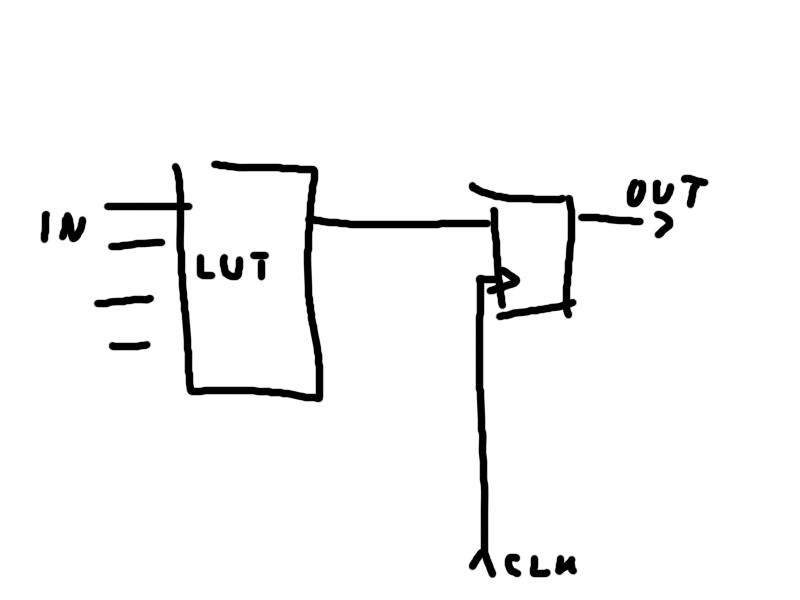
\includegraphics[width=0.7\linewidth]{slike/cell}
	\caption{}
	\label{fig:cell}
\end{figure}

\subsubsection{Kombinatorični del}
Kombinatorični del je implementiran kot iskalne tabele. To so kosi spomina, ki so sprogramirani ob zagonu vezja. V njih je sprogramirana pravilnostna tabela kombinatoričnega vezja.

\subsubsection{Spominski del}
Spominski del je implementiran kot konfigurabilna flip-flop celica, kateri lahko nastavimo polariteto, ali je zapah ali register ima reset in preset itd.


\subsection{Povezave}
Povezave zagotovijo možnost da se katera koli celica poveže z katero koli drugo celico v FPGA vezju. Matrika povezav je narejena iz mreže programibilnih križišč, ki so povezana s svojimi sosedi. Te lahko povežejo arbitrarna križišča med seboj. Na vsako križišče je povezana tudi logična celica. Taka arhitektura nam dovoli izjemno fleksibilnost a ne pride brez slabosti. Ker so povezave programibilne, pomeni, da imajo relativno veliko kapacitivnost, kar upočasni hitrost vezja.


\begin{figure}
	\centering
	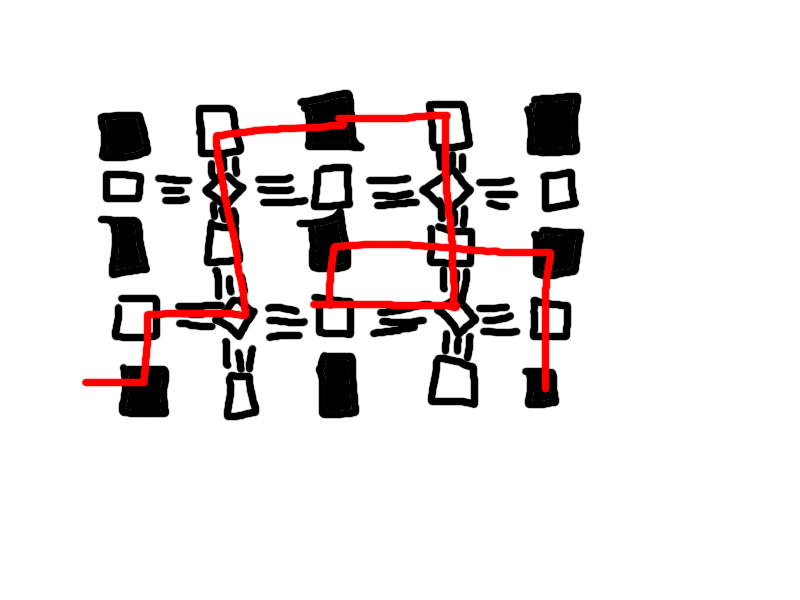
\includegraphics[width=0.7\linewidth]{slike/routing}
	\caption{}
	\label{fig:cell}
\end{figure}


\subsection{Vgrajeni bloki}
Pogosto imajo FPGA vezja tudi dodatne funkcionalnosti, ki pohitrijo pogoste primere uporabe.

\begin{itemize}
	\item \textbf{Prenosne verige}: hitre povezave med logičnimi bloki, uporabljene za ustvarjanje logike z velikim številom vhodov npr. seštevalniki
	\item \textbf{Globalne linije}: Povezave za uro in reset so ponavadi globalne, zato imajo nekatrea FPGA vezja posebne povezave za take signale. Urni signal potrebuje posebno pozornost, saj mora vse celice zadeti z čim manjšo razliko v zakasnitvah.
	\item \textbf{Specializirani bloki}: Pogosti gradniki digitalih vezji, ki zasedejo veliko prostora kot npr. množilniki in spominski bloki so ponavadi vgrajeni direktno v FPGA, da prihranimo logične celice. Nekatra FPGA vezja imajo tudi celotna procesorska jedra direktno vgrajena.
\end{itemize}



\subsection{Vhodi in izhodi}

Pomemben del FPGA vezji so tudi izhodi in vhodi. Ti so povezani na posebne bloke ki ojačajo signale, tako da so primerni za zunanje okolje. ZAgotovijo tudi sposobnost stanja visoke impedance. Pomembno je tudi, da se signali ob vstopu v vezje sinhronizirajo na notranju urni takt. Večina izhodov in vhodov so navadne digitalne povezave. Nekatera FPGA vezja imajo tudi posebne izhode in vhode za posebne protokole kot npr. PCI-E, DDR itd.



\section{Implementacija} \label{a}
Za implentacijo vezji v FPGA je potrebno spisati opis vezja v enem izmed jezikov za opis vezji(HDL). To je ponavadi (system)verilog ali VHDL. Nato programsko orodje prevede ta opis vezja v konkreten načrt tega vezja v FPGA vezju.

Cilj tega magisterskega dela je izdelava asinhronih vezji v FPGA vezjih. Problem je, da so FPGA vezja namenjena izdelavi sinhronih vezji. Velikokrat povezave med logičnimi elementi niso narejene kakor bi pričakovali, ne moramo se zanašati na zakasnitve v vezju. Večina implementacij asinhronih vezji v FPGA zato eksplicitno določi postavitev logičnih elementov in njihovih povezav v vezju. Taksen pristop deluje za manjša vezja vendar, ko vezja postanejo večja postane zelo časovno potraten. 

Namesto da ročno diktiramo povezave, da zagotovimo predpostavkam, raje uporabimo asinhroni stil, kjer so predpostavke dovolj šibke, da se lahko zanesemo, da bodo izpolnjene brez dodatnih navodil.
Zato se odločimo za dual-rail asinhroni stil. 


\subsection{SystemVerilog} \label{b}
Odločili smo se za implementacijo v jeziku SystemVerilog. Systemverilog je jezik, ki se uporablja za zasnovo in simulacijo digitalnih elektronskih vezji. Uporablja se za zasnovo vezji, ki so implementirana v FPGA.


\subsection{Knjižnica} \label{b}
Izdelali smo knjižnico v jeziku systemverilog, za izdelavo asinhronih vezji v FPGA. Knjižnica je sestavljena hierarhično

\begin{enumerate}
	\item Osnovni gradniki
	\item Funkcionalne enote
	\item Vezja
\end{enumerate}

Implementirali smo knjižnico za 4 fazen in 2 fazen stil. Kljub tem, da imajo elementi indentične vhode in izhode moramo biti pazljivi, saj štirifazna vezja ne podpirajo ciklov krajših od 3 elementov medtem, ko so lahko v dvofaznih vezjih tudi obroči z dvema elementoma.


\subsection{4-Phase dual rail} \label{b}
Štirifazna vezja implementiramo z NCL logiko. Za zapahe uporabimo mousetrap registre, ker so lepše implementirani v FPGA vezjih.

NCL logika uporablja nivojsko logiko, za izdelavo kombinatoričnih vezji. Za pravilno ponastavitev poskrbi histerezni karakter, ki poskrbi da se ničelna vrednost pravilno propagira skozi vezje.

\subsubsection{Nivojska logika} \label{c}
TODO



\subsection{2-Phase dual rail} \label{b}
Dvofazna vezja tudi uporabljajo mousetrap zapahe, vendar za kombinatorična vezja uporablja metodo bližjo naivni logični sintezi

Princip je, da zaznamo vse možne kombinacije vhodnih preklopov. Nato resetiramo te vhode in pošlenmo izhode TODO bolj natančno



\subsection{Workcraft} \label{b}
Workraft je programsko orodje za delo z grafnimi modeli. Uporabno je za zasnovo in sintezo gradnikov asinhronih vezji, kot tudi za simulacijo arhitekture raznih asinhronih vezji.

\subsubsection{Sinteza gradnikov} \label{b}
Željeno vezje opišemo z uporabo grafa signalnih preklopov(STG). V tem grafu določimo zaporedje preklopov vhodnih in izhodnih signalov, ki določajo delovanje vezja. Za C element na primer, določimo da preklopu obeh vhodov sledi preklop izhoda. Iz tega grafa orodje sestavi vezje, ki se obnaša tako kot graf, ki ga opisuje.

\subsubsection{Simulacija arhitekture asinhronih vezji} \label{b}
Za simulacijo vezji uporabimo graf signalnih preklopov(STG) oz. graf podatkovnega poteka(DFS) odvisno od stila implementacije. Za dvofazna vezja, je bolj primeren STG, saj modelira preklope, medtem ko je za štirifazna vezja bolj primeren DFS, saj upošteva ponastavitvani val, ki sledi podatkovnem valu. Te simulacije so uporabne, saj z njimi lahko preverimo, da se podatki po vezju pretakajo kot smo si to zamislisi.




\subsection{Implementacija cellic} \label{a}
Knjižnica implementira vse potrebne primitive za izdelavo poljubnih asinhronih vezji.


\subsubsection{Primitivi} \label{b}
Imamo 2 Primitiva. Primitivi so implementirani direktno z FPGA primitivi, da zagotovimo, da delujejo pravilno.

\begin{itemize}
	\item Muller C element. Klasični element implementiran z pravilnostno tableo.TODO test portable
	\item Nivojska vrata. Implemetirana direktno z pravilnostno tabelo. TODO test portable
\end{itemize}

\subsubsection{Osnovne celice} \label{b}
Osnovne celice so implementirane direktno v SystemVerilog kodi, in so prenosne na kateri koli FPGA. So najnižja stopnja v hierarhiji, zato lahko vsebujejo le druge osnovne celice.

\begin{itemize}
	\item TOGGLE. Element za dvofazna vezja. Sintetiziran s pomočjo programa workcraft. 
\end{itemize}


\subsubsection{Funkcionalne celice} \label{b}
Funkcionalne celice so sestavljene iz osnovnih celic in dodatne povezovalne logike. To so celice, ki imajo neko konkretno funkcijo kot npr. zapahi, splošni C elementi itd. 


\begin{itemize}
	\item Registri. 
\end{itemize}


\subsubsection{Logika} \label{b}
To so končani kombinatorični sklopi, ki jih lahko vmestimo direktno med registre

\begin{itemize}
	\item AND,OR. 
	\item FULL ADDER. 
	\item ect. 
\end{itemize}

\subsubsection{Vezja} \label{b}
Končana vezja, ki opravljajo določeno nalogo. Te se razlikujejo med dvofanimi in štirifaznimi implementacijamo

\begin{itemize}
	\item PIPELINE. 
	\item COUNTER. 
	\item FIBBONACCI. 
	\item GCD. 
\end{itemize}







\chapter{Rezultati} \label{rezultati}
\section{PIPELINE} \label{a}
Frekvenca, zanesljivost, meritve, ect

\section{CNT} \label{a}
Frekvenca, zanesljivost, meritve, ect

\section{FIB} \label{a}
Frekvenca, zanesljivost, meritve, ect

\section{GCD} \label{a}
Zamik, zanesljivost


\section{RISCV} \label{a}
Bomo vidl




\newpage
%******************************* ZAKLJUČEK *************************************
%******************************* ZAKLJUČEK *************************************
\chapter{Zaključek} \label{zakljucek}

Načrtali smo Asinhrona vezja in jih implementirali v FPGA. Kljub Suboptimalni arhitekturi FPGA smo dosegli delujoče rezultate in ogrodje za nadalnje delo. Hitrosti vezji so nižje kot bi upali.
	


\newpage
%******************************* LITERATURA ************************************
%******************************* LITERATURA ************************************
\cleardoublepage\phantomsection\addcontentsline{toc}{chapter}{Literatura} % vnos literature v kazalo

% 1. način: BibTeX
\bibliographystyle{ieeetrslo}
\bibliography{literatura}

% 2. način: neposreden vnos
%\begin{thebibliography}{99}
%    \bibitem{vir1} C. Su, H. Ke in T. Hubing, ``Overview of Electromagnetic Modeling Software'' [Online], v \textit{25th Annual Review of Progress in Applied Computational Electromagnetics, March 8 - March 12, 2009 - Monterey, California}. Monterey, 2009, str. 736-741. Dosegljivo: \url{http://www.clemson.edu/ces/cvel/pdf/ACES09-736.pdf}. [Dostopano: 23.8.2017].
%    \bibitem{vir2} T. Hubing et al., ``Survey of Current Computational Electromagnetics Techniques and Software'' [Online]. \textit{Clemson University Vehicular Electronics Laboratory (CVEL)}: Clemson, ZDA, CVEL-08-011.2, 21.9.2008. Dosegljivo: \url{http://www.clemson.edu/ces/cvel/Reports/CVEL-08-011.2.pdf}. [Dostopano: 23.8.2017].
%    \bibitem{vir3} \textit{The Electromagnetic Radiation Spectrum Poster} [Online]. Dosegljivo: \url{http://www.unihedron.com/projects/spectrum/}. [Dostopano: 23.8.2017].
%\end{thebibliography}
\newpage
%******************************* DODATEK ***************************************
%******************************* DODATEK ***************************************
\appendix

\chapter{Urejanje dokumentov z orodjem LaTeX} \label{prilogaA}

\begin{description}
	\item[Korak 1] Avtor kreira tekstovno datoteko s končnico \emph{.tex}, ki vsebuje tekst in ukaze za oblikovanje teksta (oziroma se uporabi izvorna koda te predloge). Dober uvod v delo z ukazi LaTeX so spletna navodila \cite{oetiker1995not}. Za pisanje je lahko uporabljen katerikoli tekstovni urejevalnik. Priporočamo uporabo urejevalnikov WinEdt\footnote{Dostopno na: http://www.winedt.org} ali TeXstudio\footnote{Dostopno na: http://texstudio.sourceforge.net/}, ki sta namenski orodji z integriranimi ikonami za posamezne korake. Urejevalnika vsebujeta tudi slovar slovenskih besed\footnote{Dostopno na: http://www.winedt.org/Dict} za sprotno preverjanje in deljenje besed. Na spletu so na voljo tudi hitri priročniki z LaTeX ukazi\footnote{Primer dostopen na: https://en.wikibooks.org/wiki/Category:Book:LaTeX} in spletni urejevalniki\footnote{Primer dostopen na: https://overleaf.com}.
	\item[Korak 2] Prevajanje izvorne datoteke s prevajalnikom MiKTeX. Možnost direktnega prevajanja v PDF dokument (ikona LaTeX) pri prvem prevajanju ustvari tudi listo citatov in sklicevanj (datoteka \emph{.aux}).
	\begin{description}
		\item[Korak 2.1]\footnote{Potrebno samo pri navajanju virov s pomočjo orodja BibTeX} Zagon BibTeX prevajanja (ikona \emph{Bib}), ki na osnovi \emph{.aux} datoteke in podatkov iz baze referenc, ustvari oblikovan spisek referenc (datoteka \emph{.bbl}) glede na izbran stil citiranja (datoteka \emph{.bst}).
		\item[Korak 2.2]\footnote{Potrebno samo pri navajanju virov s pomočjo orodja BibTeX} Ponovno prevajanje s prevajalnikom MiKTeX, ki v glavni dokument vključi oblikovane reference iz datoteke \emph{.bbl}.
	\end{description}
	\item[Korak 3] Ponovno prevajanje s prevajalnikom MiKTeX, ki poveže spisek referenc z navedki v tekstu.
	\item[Korak 4a] Pretvorba oblikovanega dokumenta v format PostScript in nato izvoz v obliki PDF dokumenta:
	\begin{itemize}[noitemsep]
		\item ikona DVI-PS - pretvorba v datoteko \emph{.ps}
		\item Ogled PostScript datoteke s programom GhostView
		\item Pretvorba v PDF dokument: GhostView: File/Convert/pdfwrite, pri čimer je potrebno izbrati parametre za format PDF/A glede na spletna navodila\footnote{Dostopno na: http://svn.ghostscript.com/ghostscript/trunk/gs/doc/Ps2pdf.htm\#PDFA}.
	\end{itemize}
	V tem primeru morajo biti vse vključene slike v formatu PostScript. V tem načinu je možna tudi uporaba orodja PSfrag, ki omogoča zamenjavo tekstovnih elementov na originalni sliki s poljubnim tekstom ali enačbo.
	\item[Korak 4b] Pretvorba oblikovanega dokumenta neposredno v PDF format. Ikona PDFTexify. V tem primeru so vključene slike lahko le v formatu PDF, PNG, JPEG ali GIF. Format izhodnega dokumenta PDF/A, ki je zahtevan za oddajo v Repozitorij UL, je podprt v tej LaTeX predlogi\footnote{Dodatne informacije: https://www.mathstat.dal.ca/\textasciitilde selinger/pdfa/}. Alternativna možnost je generiranje standardne PDF datoteke in poznejša pretvorba v format PDF/A. To je možno narediti z enim izmed plačljivih programov (npr. Adobe Acrobat Professional, Nitro Pro) ali s spletnimi pretvorniki\footnote{Primer: https://docupub.com/pdfconvert/}. Pri slednjih je potrebno biti pozoren na morebitne vodne žige ali napake, ki lahko nastanejo pri pretvorbi.
\end{description}

\chapter{Vključevanje slik v LaTeX dokumente} \label{prilogaB}

Slike vključujemo z ukazom \texttt{\textbackslash includegraphics} v okolju \texttt{figure}. EPS slike morajo biti shranjene brez glave z bitno sliko za predogled. Dodaten paket PSfrag omogoča zamenjavo (prepis) napisov na vektorski sliki. Za uporabo je potrebna vključitev orodja z ukazom \texttt{\textbackslash usepackage\{psfrag\}}. Primer LaTeX kode za zamenjavo napisa $test$ na sliki z LaTeX simbolom $\epsilon \;[\mu]$ je:

\begin{footnotesize}
	\begin{verbatim}
		\begin{figure}[h]
			\centering
			\psfrag{test}[B1][B1][1][0]{$\epsilon \;[\mu]$}
			\includegraphics[width=0.75\columnwidth]{primer_vektorske_slike.eps}
			\caption{\label{oznaka_slike} Primer slike.}
		\end{figure}
	\end{verbatim}
\end{footnotesize}

Za vključitev vektorske slike je možno uporabiti tudi makro \textbackslash epsslika, ki je vključen v stil za predlogo. Prvi parameter v makroju \textbackslash epsslika je podnaslov, drugi pa je ime datoteke s sliko brez končnice (privzeta končnica je .eps) in hkrati tudi oznaka za sklicevanje na sliko. Pri uporabi tega ukaza morajo biti datoteke EPS v korenu delovnega direktorija. Za vključevanje slika ne sme imeti glave z bitno sliko za predogled. Pri stilu je za vključevanje slik potrebno izbrati ustrezno opcijo pdftex ali pctex, glede na to katero distribucijo LaTeX prevajalnika se uporablja za prevajanje. Primer je prikazan na sliki \ref{oblika_signalov_2}.

\begin{figure}[h]
	\centering
	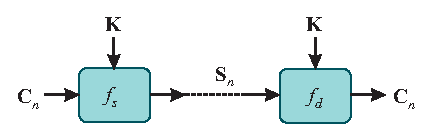
\includegraphics[width=0.75\columnwidth]{slike/vektorska_slika_2.eps}
	\caption{\label{oblika_signalov_2} Primer vektorske slike EPS.}
\end{figure}

Za vključevanje bitnih slik je v predlogi na voljo makro \textbackslash jpgslika. Prvi parameter v makroju \textbackslash jpgslika je podnaslov, drugi pa je ime datoteke s sliko (privzeta končnica je .jpg) in hkrati tudi oznaka za sklicevanje na sliko. Pri uporabi tega ukaza morajo biti slikovne datoteke v korenu delovnega direktorija. Slike so v tekst vključene v originalni velikosti.

Slika \ref{bitna_slika} predstavlja primer vključitve bitne slike JPG formata velikosti 9,4 x 7,6 cm.

\begin{figure}[h]
	\centering
	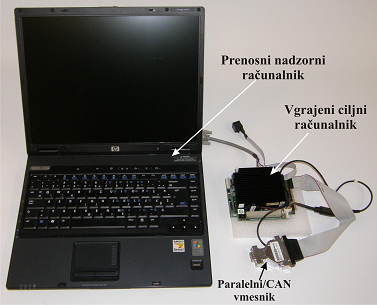
\includegraphics[width=9.4cm, height=7.6cm]{slike/bitna_slika.png}
	\caption{\label{bitna_slika} Primer vključitve bitne slike: sistem vodenja.}
\end{figure}

\chapter{Namestitev programskih orodij za urejanje LaTeX dokumentov} \label{prilogaC}

\section{Sistemi Windows}

\begin{description}
	\item[Korak 1] Namestitev paketa MiKTeX, ki je prevajalnik za dokumente, napisane v okolju LaTeX. Datoteke so dostopne na spletu: \url{http://miktex.org/}
	\item[Korak 2] Namestitev tekstovnega urejevalnika. Nekaj priporočenih:
	\begin{itemize}[noitemsep]
		\item TeXstudio (\url{http://texstudio.sourceforge.net/})
		\item Texmaker (\url{http://www.xm1math.net/texmaker/})
		\item Geany (\url{http://www.geany.org/})
		\item WinEdt (\url{http://www.winedt.com/})
	\end{itemize}
	\item[Korak 3] Namestitev ogledovalnika PostScript dokumentov:
	\begin{itemize}[noitemsep]
		\item modul GhostScript
		\item modul GhostView
	\end{itemize}
	Datoteke so dostopne na: \url{www.cs.wisc.edu/~ghost/}
\end{description}

Pri prvem prevajanju se lahko zgodi, da MiKTeX poskusi namestiti potrebne LaTeX knjižnice (pakete), kar mu je treba dovoliti, sicer predloga ne more delovati. Zaradi prenašanja in nameščanja prvo prevajanje lahko spodleti, kar je napaka paketa MiKTeX.

\section{Sistemi Linux}

Na sistemih Linux je potrebno za uporabo predloge namestiti naslednje pakete:

\begin{itemize}[noitemsep]
	\item \texttt{texlive-lang-european}
	\item \texttt{texlive-lang-greek}
	\item \texttt{texlive-latex-extra}
\end{itemize}

Imena paketov so povzeta po znani Linux distribuciji Ubuntu. V drugih distribucijah se enaki paketi lahko imenujejo tudi malo drugače. Za urejanje dokumentov se priporočajo naslednji tekstovni urejevalniki:

\begin{itemize}[noitemsep]
	\item TeXstudio (paket \texttt{texstudio})
	\item Texmaker (paket \texttt{texmaker})
	\item Geany (paket \texttt{geany})
\end{itemize}
\newpage
%%%%%%%%%%%%%%%%%%%%%%%%%%%%%%%%%%%%%%%%%%%%%%%%%%%%%%%%%%%%%%%%%%%%%%%%%%%%%%%%%%%%%%%%%%%%%%%%%%%%%%%%%%%%%%%%%%%%%%%%
\end{document}
%%%%%%%%%%%%%%%%%%%%%%%%%%%%%%%%%%%%%%%%%%%%%%%%%%%%%%%%%%%%%%%%%%%%%%%%%%%%%%%%%%%%%%%%%%%%%%%%%%%%%%%%%%%%%%%%%%%%%%%%
